\documentclass[a4paper,floatfix]{revtex4-1}
\usepackage{t1enc}
\usepackage[T1]{fontenc}
\usepackage{ulem}
\usepackage{import}
\usepackage{amsmath}
\usepackage{amssymb}
\usepackage{paralist}
\usepackage{booktabs}
\usepackage[version=3]{mhchem}
\usepackage{wrapfig}
\usepackage{pifont}
\usepackage{mathrsfs}
\usepackage{tikz}
\usepackage{xcolor}
\usepackage{color}
\usepackage{enumitem}
\usepackage{datetime}
\usepackage{textcomp}
\usepackage{relsize}
\usepackage{pgfplotstable}
%\setlist{noitemsep}
%\usepackage{lineno}
%\linenumbers

\usepackage{pgfplots}
\pgfplotsset{compat=newest}
\usepgfplotslibrary{units}
\usetikzlibrary{pgfplots.units}
\usetikzlibrary{calc}
\usetikzlibrary{spy}
\usepackage{siunitx}
%\DeclareSIUnit\molar{\mole\per\cubic\deci\metre}
%\DeclareSIUnit\textsc{M}{\textsc{M}}

\usepackage{hyperref}
\hypersetup{
 colorlinks=false,
 hidelinks=true,
}

\newcommand{\Figure}[1]{Fig.~\ref{#1}}
\newcommand{\Equation}[1]{Eqn.~\ref{#1}}
\newcommand{\Table}[1]{Tbl.~\ref{#1}}
\newcommand{\Section}[1]{Sec.~\ref{#1}}
\newcommand{\Chapter}[1]{Ch.~\ref{#1}}
\newcommand{\Appendix}[1]{Appendix~\ref{#1}}

% use roman type for natural base e and sqrt(-1)
\newcommand{\me}{{\mathrm{e}}}
\newcommand{\mi}{{\mathrm{i}}}

\definecolor{colora}{RGB}{24,90,169}
\definecolor{colorb}{RGB}{238,46,47}
\definecolor{colorc}{RGB}{0,140,72}
\definecolor{colord}{RGB}{244,125,35}
\definecolor{colore}{RGB}{61,90,153}
\definecolor{colorf}{RGB}{102,44,145}

\definecolor{tangoorange}{RGB}{245,121,0}

\newcommand{\todo}[1]{%
\textcolor{tangoorange}{#1}
}

\import{colors/}{colors}

\newsavebox\mybox{}

\begin{document}
\thispagestyle{empty}
\begin{centering}
\pgfplotsset{
 minor tick num=3,
 footnotesize,
 custom/.style={thick},
}

\begin{tikzpicture}[ baseline ]
 \pgfplotstableread{data/lowersphere10umnew.dat}{\datatablea}
 \pgfplotstableread{data/lowersphere10umnewfit.dat}{\datatableb}
 \begin{axis}[%
   %7.5000e-07
   height=250pt,width=450pt,
   xmin=-576.2676,xmax=1.9237e+03,
   %xticklabels={,,0,500,1000,1500},
   ymax=1.75,ymin=-0.6,
   axis x line*=top,
   axis y line*=right,
   ytick=\empty,
   yticklabels={,,},
   max space between ticks=40pt,
   x unit=\si{\newton\per\meter},
   xlabel=coupling $k_\mathrm{L}$,
  ]
  \draw [color=gray,dashed,semithick] (axis cs:0,1.75) -- (axis cs:0,-0.6);
 \end{axis}

 \begin{axis}[
 height=250pt,width=450pt,
 %enlargelimits=false,
 xmin=-0.12,xmax=0.40,
 ymax = 1.75,ymin=-0.6,
 %ymin=-3.25e5,ymax=8.5e5,
 xlabel=contact surface density $A_\mathrm{c}$,
 axis x line*=bottom,
 x unit=-,
 ylabel={$\Delta\!f/N_\mathrm{L}$, $\Delta\Gamma/N_\mathrm{L}$},
 y unit = \si{\hertz\meter\squared},
 %restrict x to domain = {-1e-6:2e-6},
 max space between ticks=35pt,
 %scaled x ticks = {real:1e-6},
 %xticklabel style={/pgf/number format/fixed},
 %every x tick scale label/.style={color=white},
 %legend pos = south west,
 ylabel style={yshift=-10pt},
 thick,
 %legend style={font=\tiny},
 ]
 % \newcommand\YA{5e5}
 % \newcommand\YB{-3e5}
  %\addplot [smooth,color=colora] table [ y expr=\thisrowno{1} ] {\datatablea};
  %\addlegendentry{$\Delta\!f/N_\mathrm{L}$, \SI{1}{\micro\meter}}
  %\addplot [smooth,color=colorb,
  % dash pattern={on 3pt off 0.5pt on 1pt off 0.5pt},
  %] table [ y expr=\thisrowno{2} ] {\datatablea};
  %\addlegendentry{$\Delta\Gamma/N_\mathrm{L}$, \SI{1}{\micro\meter}}

  \addplot [custom,smooth,color=colora] table [ y expr=\thisrowno{1} ] {\datatablea};
  \label{p1}
  %\addlegendentry{$\Delta\!f/N_\mathrm{L}$, sim}
  \addplot [custom,smooth,color=colorb, dash pattern={on 3pt off 0.5pt}, ] table [ y expr=\thisrowno{2} ] {\datatablea};
  \label{p2}
  %\addlegendentry{$\Delta\Gamma/N_\mathrm{L}$, sim}
  \addplot [custom,smooth,color=colora,only marks,mark=o,mark size=1pt] table [ y expr=\thisrowno{1} ] {\datatableb};
  \label{p3}
  %\addlegendentry{$\Delta\!f/N_\mathrm{L}$, theory}
  \addplot [custom,smooth,color=colorb,only marks,mark=square,mark size=1pt] table [ y expr=\thisrowno{2} ] {\datatableb};
  \label{p4}
  %\addlegendentry{$\Delta\!f/N_\mathrm{L}$, theory}

  \newcommand\YA{1}
  \newcommand\IH{60pt}
  \node[rectangle,anchor=south,draw=black,inner sep=0pt,thick] at (axis cs:-0.02,\YA)
    {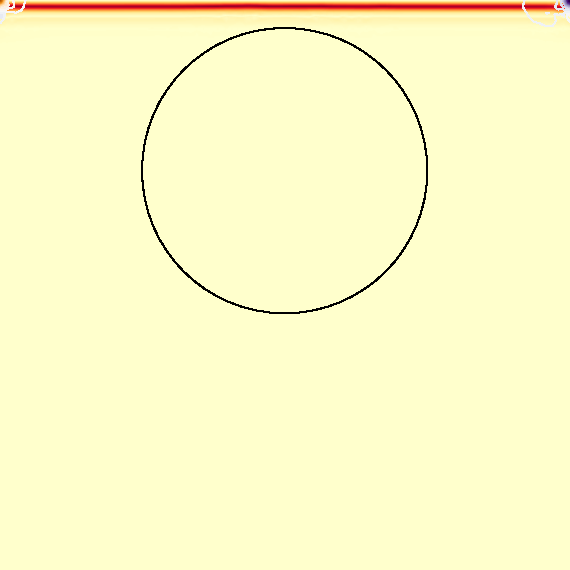
\includegraphics[angle=180,origin=c,height=\IH,keepaspectratio]{images/pu1.pdf}};
  \node[rectangle,anchor=south,draw=black,inner sep=0pt,thick] at (axis cs:0.115,\YA)
    {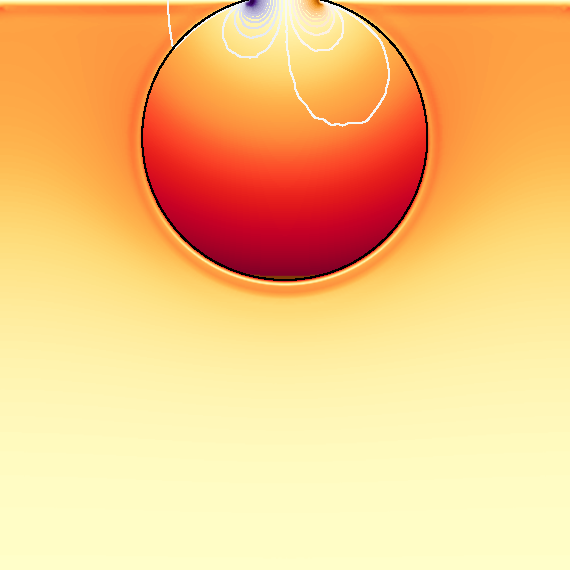
\includegraphics[angle=180,origin=c,height=\IH,keepaspectratio]{images/pu3.pdf}};
  \node[rectangle,anchor=south,draw=black,inner sep=0pt,thick] at (axis cs:0.25,\YA)
    {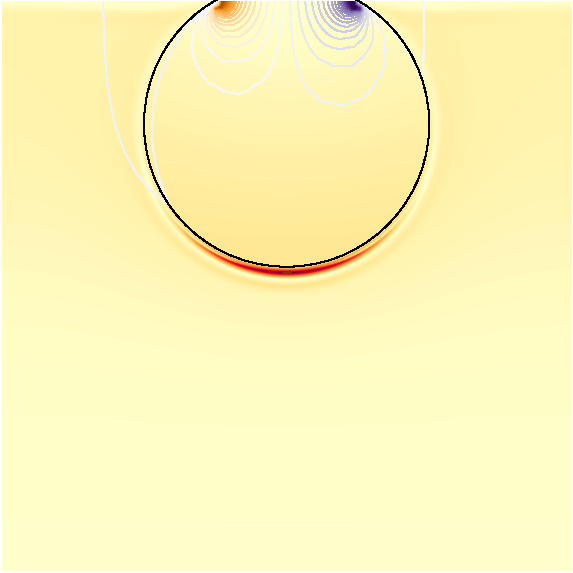
\includegraphics[angle=180,origin=c,height=\IH,keepaspectratio]{images/pu6.pdf}};

  \node[rectangle,anchor=south,draw=black,inner sep=0pt,thick] at (axis cs:0.33,\YA)
    {
\includegraphics[height={\IH-5pt},width=5px]{images/bar1.png}};
  \node[anchor=south,yshift=54pt] at (axis cs:0.33,\YA){$P$};

  \node[rectangle,anchor=south,draw=black,inner sep=0pt,thick] at (axis cs:0.35,\YA)
    {
\includegraphics[height={\IH-5pt},width=5px]{images/bar2.png}};
  \node[anchor=south,yshift=54pt] at (axis cs:0.35,\YA){$V$};

  \node[anchor=south,yshift=46pt,xshift=-23pt] at (axis cs:-0.02,\YA){\footnotesize (a)};
  \node[anchor=south,yshift=46pt,xshift=-23pt] at (axis cs:0.115,\YA){\footnotesize (b)};
  \node[anchor=south,yshift=46pt,xshift=-23pt] at (axis cs:0.25,\YA){\footnotesize (c)};

  \node [draw,fill=white,anchor=south west] at (rel axis cs: 0.01,{0.01*1.25}) {\shortstack[l]{
    \raisebox{-1.5pt}{\ref{p1}} $\Delta\!f/N_\mathrm{L}$, simulation\\
    \raisebox{-1.5pt}{\ref{p2}} $\Delta\Gamma/N_\mathrm{L}$, simulation }};

    \node [draw,fill=white,anchor=south east] at (rel axis cs: 0.99,{0.01*1.25}) {\shortstack[l]{
    \raisebox{-1.5pt}{\ref{p3}} $\Delta\!f/N_\mathrm{L}$, theory\\
    \raisebox{-1.5pt}{\ref{p4}} $\Delta\Gamma/N_\mathrm{L}$, theory}};

  %\node[anchor=south west,xshift=25pt] at (yticklabel cs:0){\includegraphics{lowerspherea.pdf}};
  %\node[anchor=south west,xshift=150pt] at (yticklabel cs:0){\includegraphics{lowersphereb.pdf}};

 \end{axis}
\end{tikzpicture}
\end{centering}


\end{document}
